\newpage

\section{Bluetooth on the CircuitPlayground Bluefruit (CPB Only) - Method4?}
\label{s:Bluetooth}

\subsection{Parts List}

\begin{enumerate}[itemsep=-5pt]
\item Smart Phone
\item Adafruit BLE Connect App (\href{https://play.google.com/store/apps/details?id=com.adafruit.bluefruit.le.connect}{Play Store}/\href{https://apps.apple.com/us/app/bluefruit-connect/id830125974}{App Store})
\item CircuitPlayground Bluefruit
\item USB Cable
\item Laptop
\end{enumerate}

\subsection{Learning Objectives}
\begin{enumerate}[itemsep=-5pt]
\item Understand the bluetooth module on the CircuitPlayground Bluefruit
\item Learn how to send data via the Bluefruit to your smart phone
\item Understand how to plot data sent via UART
\end{enumerate}

\subsection{Extra Help}

You might find plotting data via bluetooth to be rather difficult and
it was pretty difficult for me until I learned that you can export
data as a txt file rather than a csv file. Before I learned how to do
that I put together
a \href{https://www.youtube.com/playlist?list=PL_D7_GvGz-v0-U3JACRMgldvqQqn2mje9}{4
part series} describing everything in this module. Worst case you can
just watch
the \href{https://www.youtube.com/watch?v=9EHNFdVX9O8&list=PL_D7_GvGz-v0-U3JACRMgldvqQqn2mje9&index=3}{third
video in the series}. The video is 30 minutes but the first 8 minutes
goes through setting up the bluetooth module and the rest of the video
is just on plotting the exported csv data which took me some
time. Note that exporting data as a txt file is the preferred method
as parsing the file is way easier.

\subsection{Installing Modules}

{\bf One issue you're going to run into when
you run the codes below is that you won't have some of the modules on
your CPB/CPX.} To fix this you need to download
the \href{https://circuitpython.org/libraries}{CircuitPython
Libraries}. You need to download the appropriate
version: 6.x, 7.x or 8.x. How do you know what version of CircuitPython
you have? Well head over to your CIRCUITPY drive and open the
boot\_out.txt file and it will tell you the version. Note that this is
the same version as the .UF2 file installed back in the Getting
Started labs (See Chapter \ref{s:Getting_Started}). When you download
the modules it will download a .zip file. Extract the .zip file on
your desktop computer and then open the {\it lib} folder on your
desktop and your CIRCUITPY. You then need to transfer the modules
(ONLY THE ONES YOU NEED) from your desktop to your CPX/CPB {\it lib} folder. The reason
why you can't copy the entire folder is because the CPB/CPX only has
2MB of flash and the CircuitPython download is 4.1 MB at the time of
this writing. 


\subsection{Getting Started}

I mentioned in the DAQ project that there is technically a
Method4. This is because with bluetooth you can send data from your
phone to your Circuitplayground Bluefruit
(CPB) and you can also send data to your smart phone. Once
the data is on your phone you can export the data to a text file. That
basically means you can use the bluetooth module as another method to
save data from the CPB. There is a lot you can do 
with bluetooth but the bottom line is that  All
code required for this module is on
my \href{https://github.com/cmontalvo251/Microcontrollers/tree/master/Circuit_Playground/CircuitPython/CPB_DataLogger}{Github}. First we're going to run
the \href{https://github.com/cmontalvo251/Microcontrollers/blob/master/Circuit_Playground/CircuitPython/CPB_DataLogger/bluefruit_uart_button.py}{bluetooth\_uart\_button.py}
script which sends button data to your smart phone via something called UART
which is a type of serial communication. It's beyond the scope of this
lesson but serial is digital as opposed to analog which is done using the AnalogIn functions (See Chapter \ref{s:voltage})

\begin{figure}[H]
  \begin{center}
    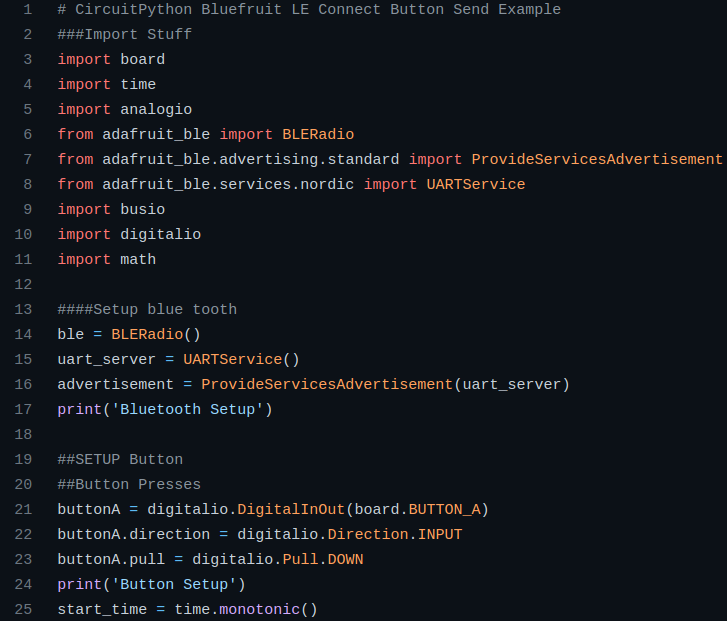
\includegraphics[width=\textwidth]{Figures/bluetooth_code.png}
  \end{center}
\end{figure}
Lines 3-11 import a ton of modules. You'll recognize many of them like
analogio, and time but the new ones are the ones that
say ble. These are the bluetooth modules required for the CPB. Lines
21-24 setup the button so we can log the button via bluetooth and
Lines 14-17 kick of the BLERadio object and the UARTService() to send
data. Line 25 also grabs the current time before the infinite while
loop that way the timer starts closer to zero. 
\begin{figure}[H]
  \begin{center}
    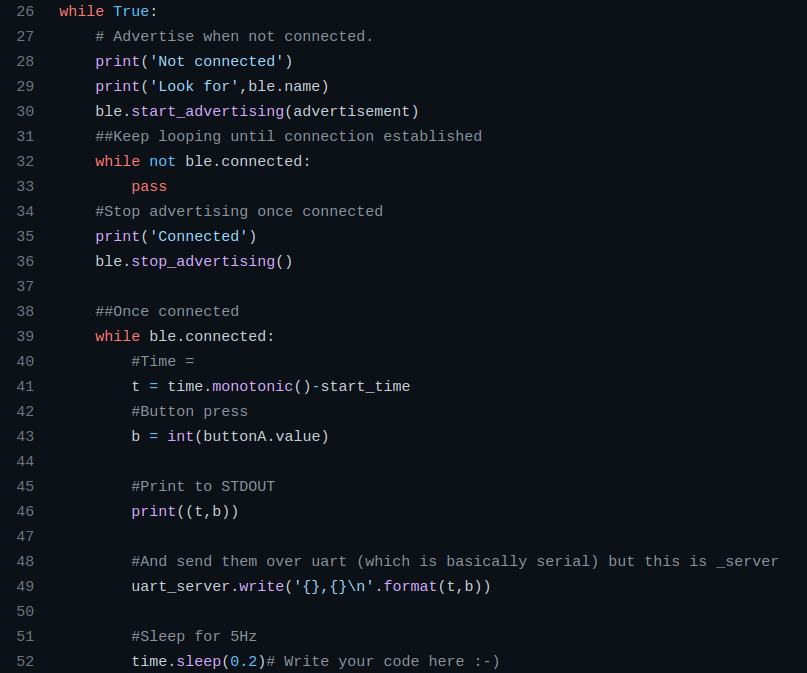
\includegraphics[width=\textwidth]{Figures/bluetooth_code1.png}
  \end{center}
\end{figure}
The code above is the infinite while loop which actually contains 2
while loops. Lines 28-33 prints the name of your bluetooth sensor and
then starts advertising bluetooth to whoever is listening. It will
then enter a while loop from 32-33 until 
bluetooth is connected. Once bluetooth is connected it will enter into
the second while loop from line 39-52. In those lines 40-46 is
responsible for taking all the necessary measurements and printing
them to the serial monitor in Mu. In this case it's only printing the
current time and the value of the button as an integer. {\it
buttonA.value} is either True or False and the {\it int} function
converts that to a 0 or a 1. Line 49 then sends the data
over bluetooth using the UART server. You'll notice in this case the
code is sending t,b by
using the format variable and the 2 empty {} brackets. If you want to
send more data you need to add more empty brackets and more variables
to the format function. When you first save this script your CPB will
not be connected and enter into an infinite while loop where it waits
for your smart phone to connect. If you open your smart phone and open
the Bluefruit Connect App the following screen will pop up. 
\begin{figure}[H]
  \begin{center}
    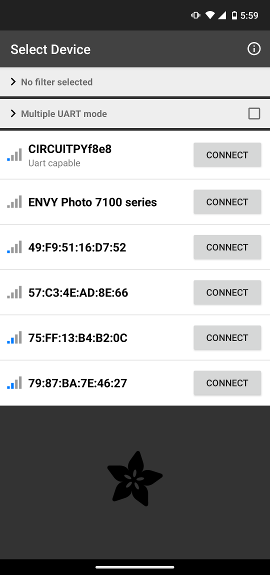
\includegraphics[width=0.3\textwidth]{Figures/phoneapp1.png}
  \end{center}
\end{figure}
In this case there are numerous different bluetooth modules can be
seen but the one you need to click is the one that says
CIRCUITPYf8e8. You will have a different code after CIRCUITPY and you
can figure out what your 4 digit code is by making sure you have the
{\it print('Look for',ble.name)} in your code. Once you do that the
CPB will begin sending time and the button press to your smart phone. 
\begin{figure}[H]
  \begin{center}
    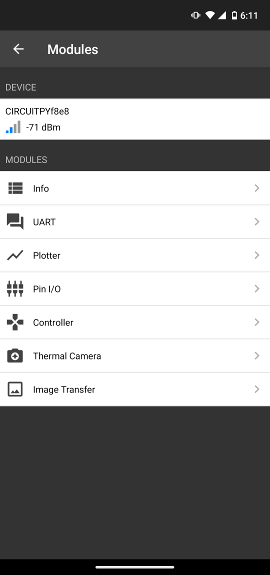
\includegraphics[width=0.3\textwidth]{Figures/phoneapp2.png}
  \end{center}
\end{figure}
There are numerous items you can click. The Controller is very fun for
creating a remote control robot but we're only going to go over the
UART and Plotter tabs. If you click the plotter tab you will be
greeted with a live screen of the data being sent. 
\begin{figure}[H]
  \begin{center}
    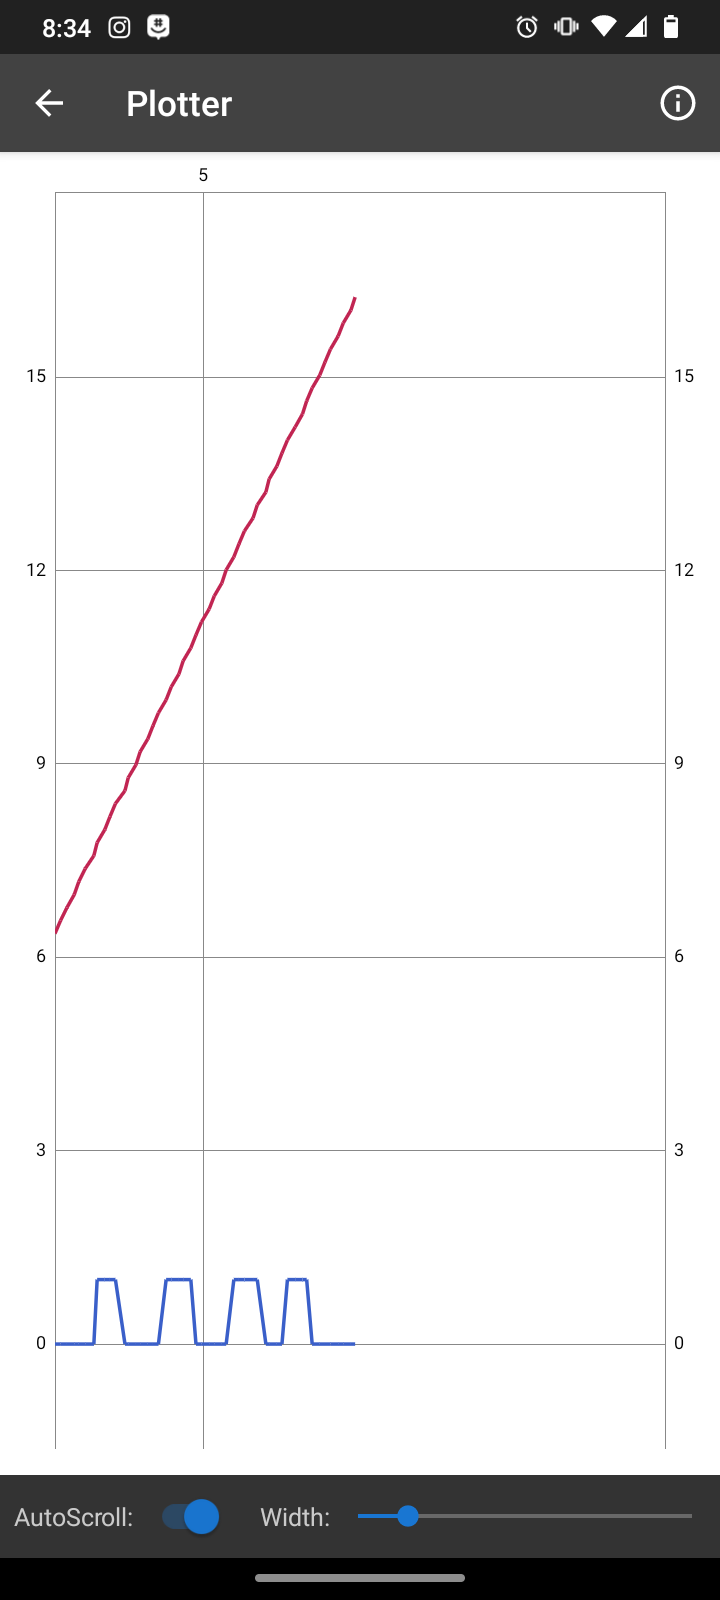
\includegraphics[width=0.3\textwidth]{Figures/phoneapp3.png}
  \end{center}
\end{figure}
In the photo above you can see three data streams that is coming
directly from the CPB. The red line is time and the blue line is the
button value. Notice the blue line goes from 0 to 1 which means I
pressed the button a few times. The red line is always increasing
which kind of messes up the plotter so you can always go back to your
code in Mu and just send your data. This is great for live demonstrations and for
debugging if you need to see data from an experiment and you don't
have access to a laptop with Mu. If you hit the back arrow and then
click UART you will see the raw data come in as text. 
\begin{figure}[H]
  \begin{center}
    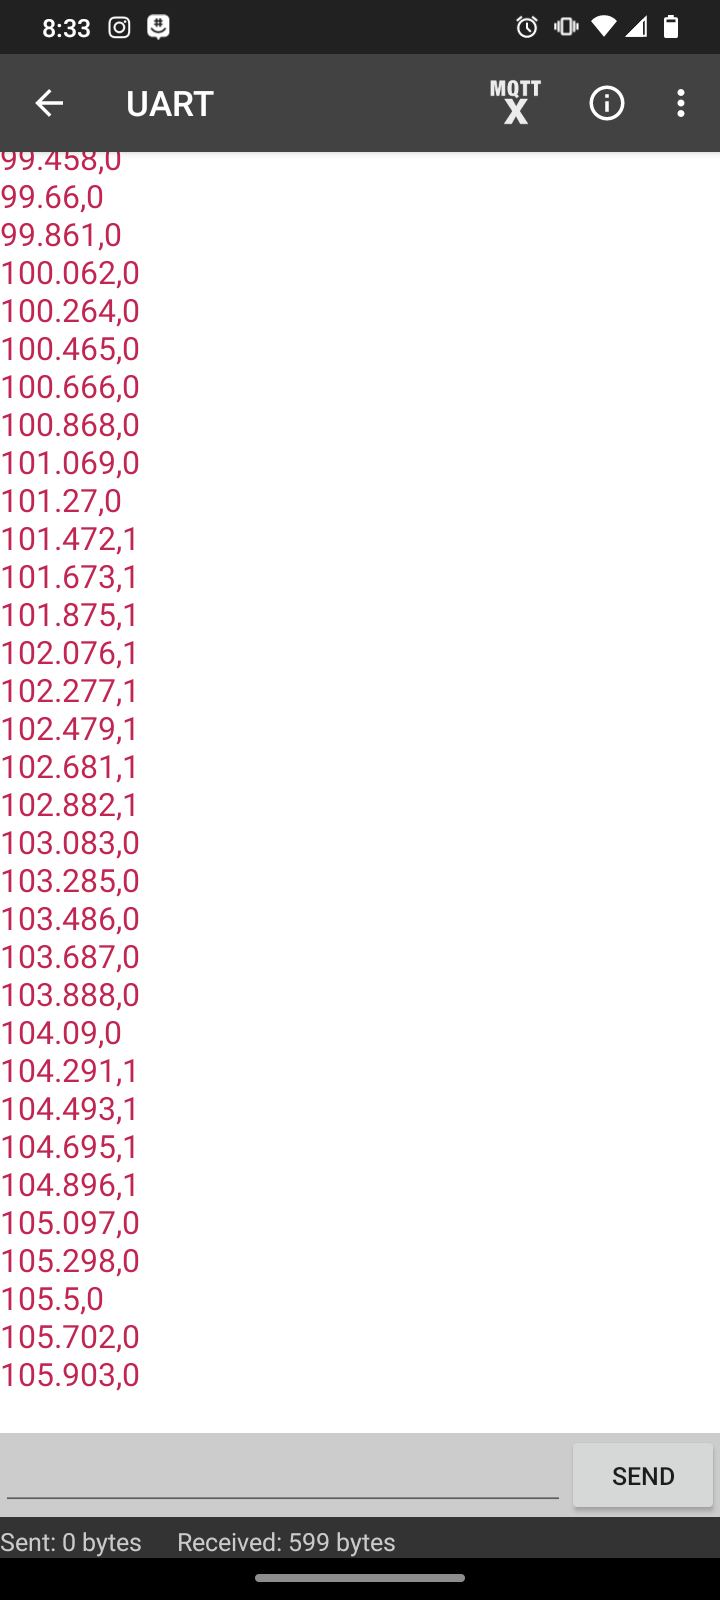
\includegraphics[width=0.3\textwidth]{Figures/phoneapp4.png}
  \end{center}
\end{figure}
Again here you can see the 3 data streams separated by commas. The
very neat thing with the UART tab is that you can click the three
vertical dots in the upper right hand corner and click export to
TXT. The easiest thing for me was to export the data to google drive
and then download the data to my computer. Once I downloaded the TXT file to my
computer and opened it the data file looked like this. 
\begin{figure}[H]
  \begin{center}
    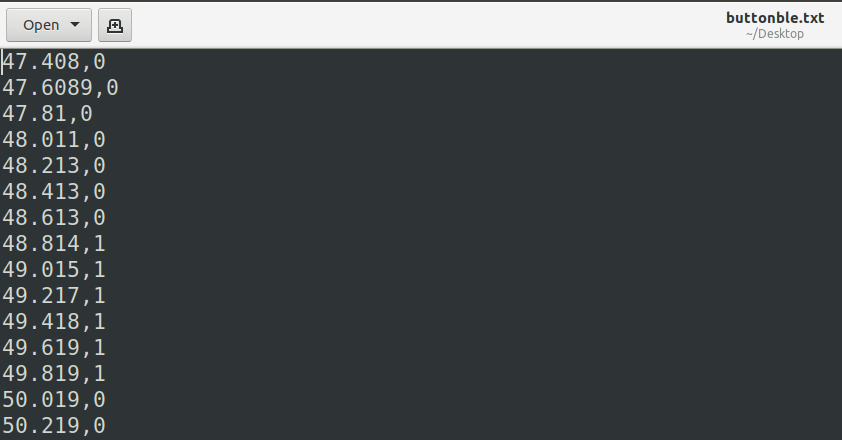
\includegraphics[width=0.8\textwidth]{Figures/csv_fileapp.png}
  \end{center}
\end{figure}
If you export the file as a CSV the data file will look completely
different and it's much more complicated to plot. If you export the
data as a TXT file you just need to use the np.loadtxt command to read
in the data. Note you might have commas in your data file. If there
are commas just use the CTRL+H command and replace all commas with
spaces or use the np.loadtxt('buttonble.txt',delimiter=',')
command. Plotting your button presses should be as simple as the
previous lab thus plotting the button is left as an exercise to the
reader. 

\subsection{Assignment}

Once you've completed the project above, upload a PDF with all of the photos and text
below included. My recommendation is for you to create a Word document
and insert all the photos and text into the document. Then export the
Word document to a PDF. For videos I suggest uploading the videos to
Google Drive, turn on link sharing and include a link in your
PDF. {\bf Note that all code must be included in the appendix or you'll be
penalized 10\%.}
\ \\

{\bf For all videos you must explain what you're doing. At a minimum state your name and explain what your circuit does.}


\begin{enumerate}[itemsep=-5pt]
\item First get the bluetooth code on your CPB and connect your smart phone to it and video tape yourself connecting the CPB to your smart phone (20\%)
\item Take a screenshot of the Plotter on your phone (15\%)
\item Take a screenshot of the UART raw data on your phone (15\%)
\item Export time, and button presses to a TXT file and plot it on
your computer. Include your raw data in an appendix. (20\%)
\item Include a plot of your button presses with time on the x-axis
and button value on the y-axis (30\%)
\end{enumerate}
